%%%%%%%%%%%%%%%%%%%%%%%%%%%%%%%%%%%%%%%%%%%%%%
% Head matter - can we try to be consistent on
% included packages
\ifdefined\beamerclass
\else
    \def\beamerclass{beamer}
\fi
\documentclass[\beamerclass]{beamer}

\usepackage{pgfpages}
\mode<handout>{
	% \setbeamercolor{background canvas}{bg=black!20}
	\pgfpagesuselayout{2 on 1}[a4paper,border shrink=5mm]
}

%\documentclass{beamer}
\mode<presentation>
{\usetheme{default}
 \usecolortheme{default}
 \usefonttheme{default}
 \setbeamertemplate{navigation symbols}{}
 \setbeamertemplate{footline}[frame number]
% \setbeamertemplate{caption}[numbered]
 }
\usepackage[english]{babel}
\usepackage{algorithm}
\usepackage[noend]{algpseudocode}
\usepackage[utf8x]{inputenc}
\usepackage{graphicx}
\usepackage{hyperref}
%\graphicspath{{./images/}}
\usepackage{tikz}
\usetikzlibrary{shapes.geometric, arrows,chains}
\usepackage{booktabs,makecell,multirow,tabularx}
\usepackage{verbatim}
\renewcommand{\arraystretch}{1.2}
\renewcommand\theadfont{\normalfont\bfseries}
\usepackage{array}
\usepackage{listings}
\lstset{language=Java, showstringspaces=false}
\usepackage[normalem]{ulem}
\usepackage{bm}
\def\layersep{2.5cm}

\usepackage{xcolor}
%\usepackage{subfig}
\setbeamertemplate{caption}{\insertcaption}
\usepackage[caption=false]{subfig}
\usepackage{hyperref}
\usepackage{verbatim}

\usetheme{Copenhagen}
\hypersetup{pdfstartview={Fit}}
\lstset{basicstyle=\small\ttfamily,breaklines=true}

\usepackage{xmpmulti}

%\setbeamertemplate{caption}[numbered]%\numberwithin{figure}{section}
% Define block styles
\tikzstyle{decision} = [diamond, draw, fill=blue!20, 
    text width=4.5em, text badly centered, node distance=3cm, inner sep=0pt]
\tikzstyle{block} = [rectangle, draw, fill=blue!20, 
    text width=3em, text centered, rounded corners, minimum height=3em]
\tikzstyle{line} = [draw, -latex']
\tikzstyle{cloud} = [draw, ellipse, fill=red!20, node distance=3cm,
    minimum height=2em]
\tikzset{
  startstop/.style={
    rectangle, 
    rounded corners,
    minimum width=3cm, 
    minimum height=1cm,
    align=center, 
    draw=black, 
    fill=red!30
    },
  process/.style={
    rectangle, 
    minimum width=3cm, 
    minimum height=1cm, 
    align=center, 
    draw=black, 
    fill=blue!30
    },
  decision/.style={
    rectangle, 
    minimum width=3cm, 
    minimum height=1cm, align=center, 
    draw=black, 
    fill=green!30
    },
  arrow/.style={thick,->,>=stealth},
  dec/.style={
    ellipse, 
    align=center, 
    draw=black, 
    fill=green!30
    },
}
\tikzstyle{arrow} = [thick,->,>=stealth]

\tikzset{onslide/.code args={<#1>#2}{%
  \only<#1>{\pgfkeysalso{#2}} % \pgfkeysalso doesn't change the path
}}

\makeatletter
\newenvironment<>{btHighlight}[1][]
{\begin{onlyenv}#2\begingroup\tikzset{bt@Highlight@par/.style={#1}}\begin{lrbox}{\@tempboxa}}
{\end{lrbox}\bt@HL@box[bt@Highlight@par]{\@tempboxa}\endgroup\end{onlyenv}}

\newcommand<>\btHL[1][]{%
  \only#2{\begin{btHighlight}[#1]\bgroup\aftergroup\bt@HL@endenv}%
}
\def\bt@HL@endenv{%
  \end{btHighlight}%   
  \egroup
}
\newcommand{\bt@HL@box}[2][]{%
  \tikz[#1]{%
    \pgfpathrectangle{\pgfpoint{1pt}{0pt}}{\pgfpoint{\wd #2}{\ht #2}}%
    \pgfusepath{use as bounding box}%
    \node[anchor=base west, fill=orange!30,outer sep=0pt,inner xsep=1pt, inner ysep=0pt, rounded corners=3pt, minimum height=\ht\strutbox+1pt,#1]{\raisebox{1pt}{\strut}\strut\usebox{#2}};
  }%
}
\makeatother

\definecolor{darkblue}{RGB}{37,55,97}
\definecolor{mellowyellow}{RGB}{247,206,70}
\definecolor{almostwhite}{RGB}{254,255,255}
\definecolor{merrygreen}{RGB}{79,173,91}
\definecolor{funkyorange}{RGB}{240,154,56}

\addtobeamertemplate{footnote}{\hskip -2em}{}
\newcommand\blfootnote[1]{%
  \begingroup
  \renewcommand\thefootnote{}\footnote{#1}%
  \addtocounter{footnote}{-1}%
  \endgroup
}

\DeclareMathOperator{\softmax}{softmax}
\DeclareMathOperator{\ReLU}{ReLU}

%%%%%%%%%%%%%%%%%%%%%%%%%%%%%%%%%%%%%%%%%%%%%%
% Formatting for title page
\title[RNNs]{Recurrent Neural Networks}
\author{Jonathon Hare}
\institute[]
{
  Vision, Learning and Control\\
  University of Southampton 
}
\date{}
\subject{Computer Science}
\useoutertheme{infolines}
\setbeamertemplate{headline}{} %remove headline
\setbeamertemplate{navigation symbols}{} %remove navigation symbols
%%%%%%%%%%%%%%%%%%%%%%%%%%%%%%%%%%%%%%%%%%%%%%
\begin{document}

\begin{frame}[plain]
        \begin{tikzpicture}[overlay, remember picture, shift={(current page.south west)},font={\fontfamily{Montserrat-TOsF}\selectfont}]
        \fill [mellowyellow,text=darkblue] (0,0) rectangle (\paperwidth, \paperheight);
        \draw (4,7) node [align=left,text=darkblue] {\Huge \begin{tabular}{l} \textbf{Process} \\ \textbf{Sequences} \end{tabular}};
        \draw (11,1) node [align=left,text=darkblue] {\includegraphics[scale=0.15]{../vlc.png}};
        \end{tikzpicture}
\end{frame}

\begin{frame}
  \titlepage

  \tiny{A lot of the ideas in this lecture come from Andrej Karpathy's blog post on the Unreasonable Effectiveness of RNNs (\url{https://medium.com/@karpathy/yes-you-should-understand-backprop-e2f06eab496b}). Many of the images and animations and were made by Adam Pr\"ugel-Bennett.}
\end{frame}
%-------------------------------------------------------------%


\begin{frame}[fragile]{pause}\frametitle{Recurrent Neural Networks - Motivation}
\begin{center}

\begin{tabular}{ c c c c c c c c}
$x$: & Jon & and & Ethan & gave & deep & learning & lectures\\ \\
$y$: & 1 & 0 & 1 & 0 & 0 & 0 & 0 \\
\end{tabular}
\end{center}
\end{frame}
%-------------------------------------------------------------%

\begin{frame}{pause}\frametitle{Recurrent Neural Networks - Motivation}
\begin{center}
\begin{tabular}{ c c c c c c }
$x$: & $x^{(1)}$ & ... & $x^{(t)}$ & ... & $x^{(T_x)}$ \\
$x$: & Jon & ... & Ethan & ... & lectures \\ \\
$y$: & $y^{(1)}$ & ... & $y^{(t)}$ & ... & $y^{(T_y)}$ \\
$y$: & 1 & ... & 1 & ...& 0 \\ \\ \\
\end{tabular}
\end{center}

In this example, $T_x = T_y = 7$ but $T_x$ and $T_y$ can be different.
\end{frame}
%-------------------------------------------------------------%

\begin{frame}[fragile]\frametitle{Recurrent Neural Networks}
\center{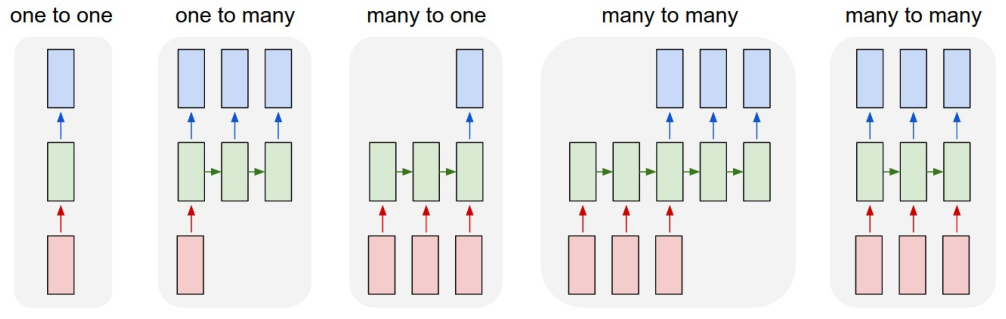
\includegraphics[width=0.99\textwidth]{seqmods.pdf}}  \blfootnote{Image from \url{http://karpathy.github.io/2015/05/21/rnn-effectiveness/}}
\end{frame}

%-------------------------------------------------------------%

\begin{frame}[fragile]\frametitle{Aside: One Hot Encoding}

How can we represent individual words (or other discrete tokens)?
\center{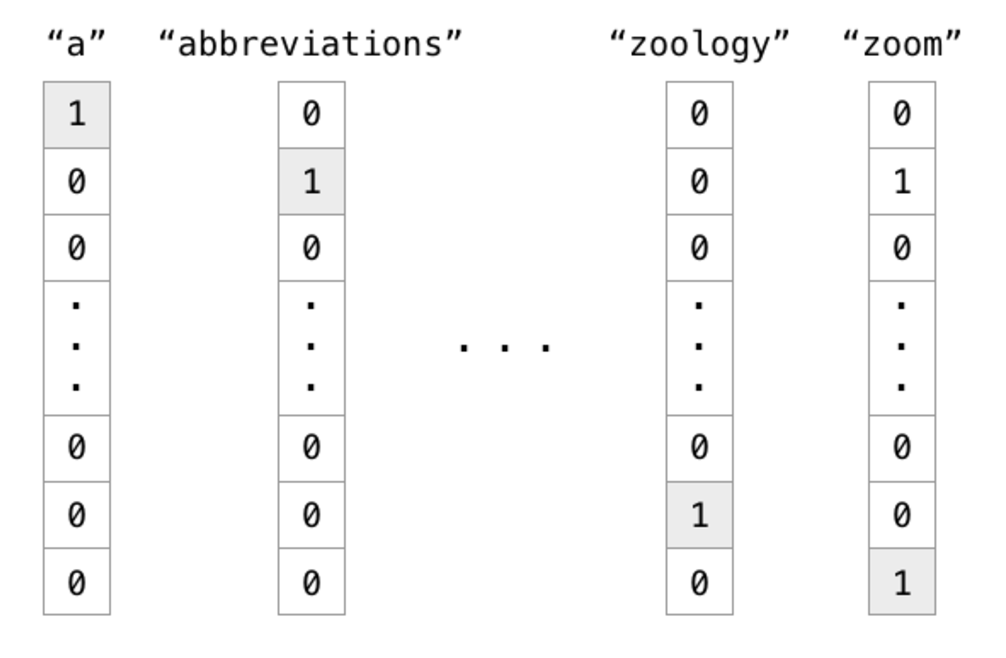
\includegraphics[width=0.9\textwidth]{onehot.pdf}\blfootnote{Image from \url{https://ayearofai.com}}}
\end{frame}
%-------------------------------------------------------------%

\begin{frame}\frametitle{Why Not a Standard Feed Forward Network?}
\begin{itemize}
\item<+-> For a task such as ``Named Entity Recognition'' a MLP would have several disadvantages
\begin{itemize}
  \item<+-> The inputs and outputs may have varying lengths
  \item<+-> The features wouldn't be shared across different temporal positions in the network
  \begin{itemize}
    \item<+-> Note that 1-D convolutions can be (and are) used to address this, in addition to RNNs - more on this in a later lecture
  \end{itemize}
\end{itemize}
\item<+-> To interpret a sentence, or to predict tomorrows weather it is necessary to remember what happened in the past
\item<+-> To facilitate this we would like to add a feedback loop delayed in time
\end{itemize}
\end{frame}
%-------------------------------------------------------------%

\begin{frame}[fragile]{pause}\frametitle{Recurrent Neural Networks}
\center{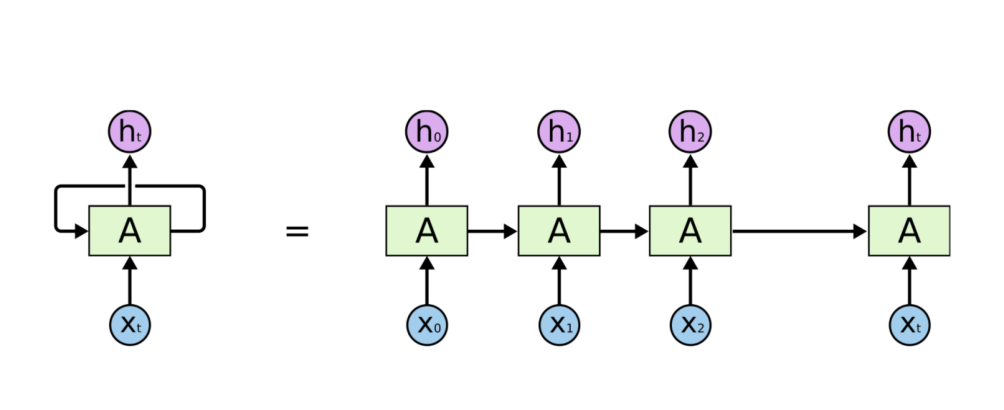
\includegraphics[width=0.99\textwidth]{rnn1.pdf}\footnote{Image taken from \url{https://towardsdatascience.com}}}
\begin{itemize}
\item RNNs are a family of ANNs for processing sequential data \pause
\item RNNs have directed cycles in their computational graphs 
\end{itemize}
\end{frame}
%-------------------------------------------------------------%

\begin{frame}[fragile]{pause}\frametitle{Recurrent Neural Networks}
RNNs combine two properties which make them very powerful.
\begin{enumerate}
\item Distributed hidden state that allows them to store a lot of information about the past efficiently. This is because several different units can be active at once, allowing them to remember several things at once.
\item Non-linear dynamics that allows them to update their hidden state in complicated ways\footnote{Often said to be difficult to train, but this is not necessarily true - dropout can help with overfitting for example}.
\end{enumerate}

\end{frame}
%-------------------------------------------------------------%
\begin{frame}[fragile]{pause}\frametitle{Recurrent Neural Networks}
RNNs are Turing complete in the sense they can simulate arbitrary programs\footnote{Don't read too much into this - like universal approximation theory, just because they can doesn't mean its necessarily learnable!}. \pause
\begin{block}{}
  \center
  If training vanilla neural nets is optimisation over functions, training recurrent nets is optimisation over programs.
\end{block}
\end{frame}
%-------------------------------------------------------------%

\begin{frame}
\frametitle{Recurrent Network}
\begin{center}
  \multiinclude[<+>][format=pdf, graphics={width=\linewidth}] {recurrent}
\end{center}
\end{frame}

%-------------------------------------------------------------%

\begin{frame}{pause}
\frametitle{Training Recurrent Networks}

\begin{itemize}
\item Given a set of inputs $\mathcal{D} = 
  \left((\bm{x}(t), \bm{y}(t)) \big\vert t=1,\,2,\,\ldots,\, T \right)$\pause
\end{itemize}
\begin{center}
  \only<-9>{
  \multiinclude[<+>][format=pdf, graphics={width=\linewidth}] {bptt}
  }
  \includegraphics<+->[width=\linewidth]{bptt-7.pdf}
\end{center}
\begin{itemize}
\item Minimise an error (here MSE, but your choice):
  \begin{align*}
    E(\bm{W}) = \sum_{t=1}^T \left\| \bm{y}(t)
    - \bm{f}(\bm{x}(t), \bm{c}(t-1)|\bm{W}) \right\|^2
  \end{align*}\pause
\item This is known as \emph{back-propagation through time}\pause
\end{itemize}

\end{frame}

%-------------------------------------------------------------%

%% Just show it as a recursive invokation of the chain rule...
\begin{frame}
\frametitle{An RNN is just a recursive function invocation}

\begin{itemize}
  \item<+-> $\bm{y}(t) = \bm{f}(\bm{x}(t), \bm{c}(t-1)|\bm{W})$
  \item<+-> and the state $\bm{c}(t) = \bm{g}(\bm{x}(t-1), \bm{c}(t-1)|\bm{W})$
  \item<+-> If the output $\bm{y}(t)$ depends on the input
    $\bm{x}(t-3)$, then prediction will be
    \begin{align*}
      \bm{f}(\bm{x}(t), \bm{g}(\bm{x}(t-1), \bm{g}(\bm{x}(t-2), \bm{g}(\bm{x}(t-3)|\bm{W}), \bm{W}), \bm{W}), \bm{W})
    \end{align*}
  \item<+-> it should be clear that the gradients of this with respect to the weights can be found with the chain rule
\end{itemize}

\end{frame}


%-------------------------------------------------------------%

%%  Introduce the internals - basically how all variants are the same structure with different update rules
%% Vanilla  RNN - Elman Network
\begin{frame}
\frametitle{What is the state update $g()$?}

\begin{itemize}
  \item<+-> It depends on the variant of the RNN!
  \begin{itemize}
    \item Elman
    \item Jordan
    \item LSTM
    \item GRU
  \end{itemize}
\end{itemize}

\end{frame}

%-------------------------------------------------------------%

\begin{frame}
\frametitle{Elman Networks (``Vanilla RNNs'')}

\begin{align*}
  \bm h_t &= \sigma_h(\bm W_{ih} \bm x_t + \bm b_{ih} + \bm W_{hh} \bm h_{t-1} + \bm b_{hh}) \\
  \bm y_t &= \sigma_y(\bm W_{y} \bm h_t + \bm b_y)
\end{align*}

\only<2-> {
\begin{itemize}
  \item $\sigma_h$ is usually $\tanh$
  \item $\sigma_h$ is usually identity (linear) -- the $y$'s could be regressed values or logits
  \item<+-> the state $\bm h_t$ is referred to as the ``hidden state''
  \item<+-> the output at time $t$ is a projection of the hidden state at that time
  \item<+-> the hidden state at time $t$ is a summation of a projection of the input and a projection of the previous hidden state
\end{itemize}
}
\end{frame}

%-------------------------------------------------------------%

\begin{frame}
\frametitle{Going deep: Stacking RNNs}

\end{frame}

%-------------------------------------------------------------%

% End with an example: char-level language modelling

\begin{frame}
\frametitle{Example: Character-level language modelling}

\end{frame}

\begin{frame}
\frametitle{Sampling the Language Model}

\end{frame}

\end{document}
